\documentclass[a4paper, 11pt]{article}
\usepackage{graphicx}
\usepackage{amsmath}
\usepackage[pdftex]{hyperref}

% Lengths and indenting
\setlength{\textwidth}{16.5cm}
\setlength{\marginparwidth}{1.5cm}
\setlength{\parindent}{0cm}
\setlength{\parskip}{0.15cm}
\setlength{\textheight}{22cm}
\setlength{\oddsidemargin}{0cm}
\setlength{\evensidemargin}{\oddsidemargin}
\setlength{\topmargin}{0cm}
\setlength{\headheight}{0cm}
\setlength{\headsep}{0cm}

\renewcommand{\familydefault}{\sfdefault}

\title{Machine Learning 2014: Project 1 - Regression Report}
\author{member1@student.ethz.ch\\vlucas@student.ethz.ch\\ piusv@studemY nt.ethz.ch\\}
\date{\today}

\begin{document}
\maketitle

\section*{Experimental Protocol}
%Suppose that someone wants to reproduce your results. Briefly describe the steps used to obtain the
%predictions starting from the raw data set downloaded from the project website. Use the following
%sections to explain your methodology. Feel free to add graphs or screenshots if you think it's
%necessary. The report should contain a maximum of 2 pages.

\section{Tools}
%Which tools and libraries have you used (e.g. Matlab, Python with scikit-learn, Java with Weka,
%SPSS, language x with library y, $\ldots$). If you have source-code (Matlab scripts, Python scripts, Java source folder, \dots),
%make sure to submit it on the project website together with this report. If you only used
%command-line or GUI-tools describe what you did.

We exclusively used $Matlab$ for this assignment.
We used $csvread$ to read the provided training and validation data sets and
$csvwrite$ to write our predictions. For regression and crossvalidation we used
the $lasso$ function. The $plot$ function was also useful for data exploration
and guessing useful non-linear feature transformations. The figure in section $4$
was created with $lassoPlot$.


\section{Algorithm}
%Describe the algorithm you used for regression (e.g. ordinary least squares, ridge regression, $\ldots$)
We used $L1$ regularized least squares regression provided by the $lasso$ function in $Matlab$.

\section{Features}
%Did you construct any new features? What feature transforms did you use?

From the original set of $14$ features $\left\{x_1, x_2, \ldots, x_{14} \right\}$
we constructed the new features
\[
\left\{z_1, \ldots z_5, z_{1}^{2}, z_1z_2, \ldots, z_4z_5, z_{5}^{2}, z_{1}^{3}, z_{2}^{3}, \ldots, z_{5}^{3} \right\}
\]
where $z_1 = \frac{1}{x_1}$, $z_2 = x_2$, $z_3 = x_4$, $z_4 = \frac{1}{x_6}$, $z_5 = x_{14}$.

\section{Parameters}
%How did you find the parameters of your model? (What parameters have you searched over, cross validation procedure, $\ldots$)

We used lasso regression with 10 fold cross validation to determine our model parameters.
The $lasso$ function provided by $Matlab$ allows us to do so easily. Additionally it lets
us find the $L1$ penalty parameter $\lambda$ which gives the lowest expected cross validation error.

\begin{center}
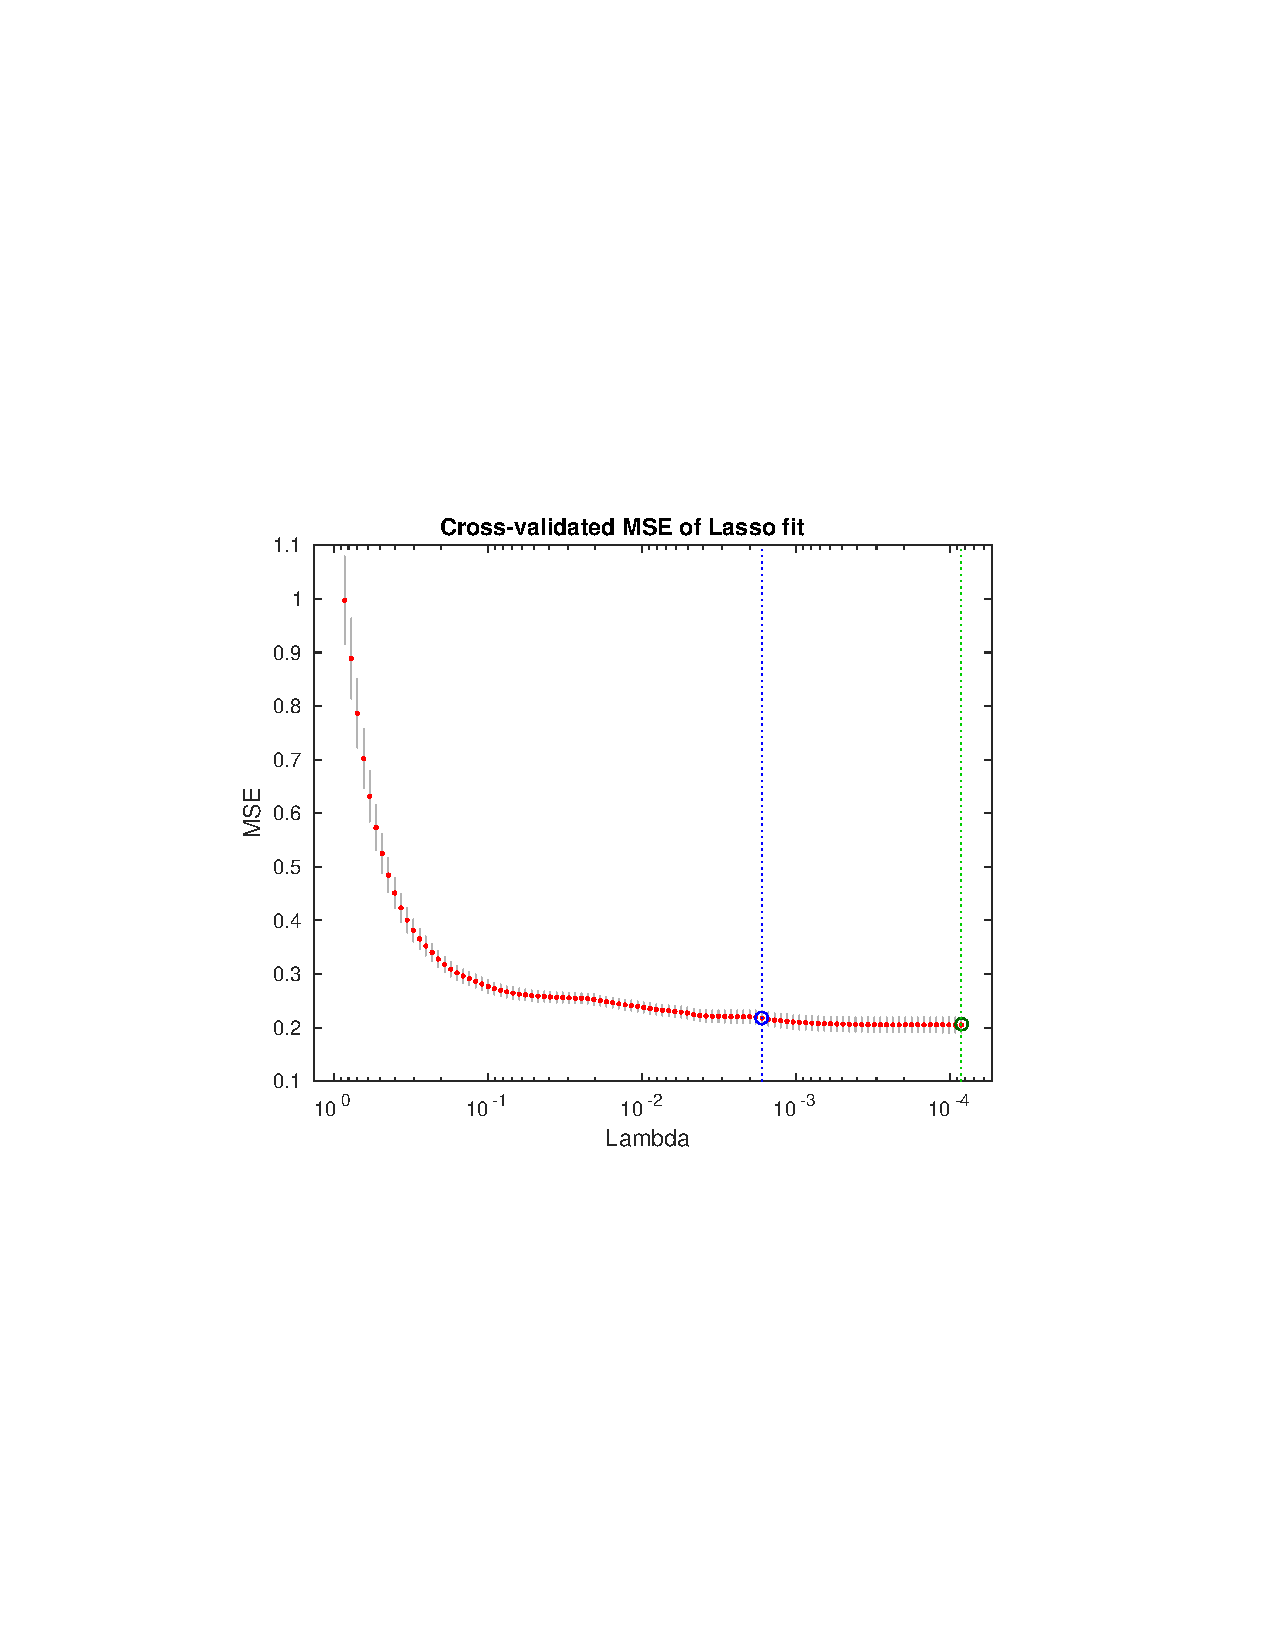
\includegraphics[width=5in]{lasso_mse}
\end{center}

\section{Lessons Learned}
%What other algorithms, tools or methods did you try out that didn't work well?
%Why do you think they performed worse than what you used for your final submission?

Additionally to lasso regression we tried training a Neural Network (provided by a $Matlab$ toolbox) and
Gaussian Process regression (using the open source $GPML$ library). They both
seemed to perform worse because of a lack of additional training data.

\end{document}
